%                                                                aa.dem
% AA vers. 9.1, LaTeX class for Astronomy & Astrophysics
% demonstration file
%                                                       (c) EDP Sciences
%-----------------------------------------------------------------------
%
%\documentclass[referee]{aa} % for a referee version
%\documentclass[onecolumn]{aa} % for a paper on 1 column  
%\documentclass[longauth]{aa} % for the long lists of affiliations 
%\documentclass[letter]{aa} % for the letters 
%\documentclass[bibyear]{aa} % if the references are not structured 
%                              according to the author-year natbib style

%
\documentclass{aa}  

%
\usepackage{graphicx}
%%%%%%%%%%%%%%%%%%%%%%%%%%%%%%%%%%%%%%%%
\usepackage{txfonts}
\usepackage{xcolor}
%%%%%%%%%%%%%%%%%%%%%%%%%%%%%%%%%%%%%%%%
\usepackage{hyperref}
% To add links in your PDF file, use the package "hyperref"
% with options according to your LaTeX or PDFLaTeX drivers.
%
\begin{document} 

\def\simgt{\lower.5ex\hbox{$\; \buildrel > \over \sim \;$}}
\def\simlt{\lower.5ex\hbox{$\; \buildrel < \over \sim \;$}}
\def\etal{{\it et al.}}
\def\msun{M$_\odot$}
\def\Msun{M$_\odot$}
\def\rsun{R$_\odot$}
\def\Teff{$T_{\rm eff}~$}
\def\teff{$T_{\rm eff}$}
\def\BMV{$B-V$~}
\def\EBV{$E_{B-V}$}
\def\dv{$\Delta V$~}
\def\Mc{$M_\rm c$~}
\def\X{$X$~}
\def\FeH{${\rm [Fe/H]}$~}
\def\feh{${\rm [Fe/H]}$}
\def\Y{$Y$~}
\def\Z{$Z$~}
\def\Lto{$L_{\rm TO}$~}
\def\Hp{$H_{\rm p}$~}
\def\logL{$\log (L/L_{\odot})$~}
\def\Mv{$M_{\rm v}$~}
\def\M{$M$}
\def\R{$R$}
\def\alfamlt{$\alpha_{\rm MLT}$~}
\def\alfaatm{$\alpha_{\rm atm}$~}
\def\alfa2d{MLT--$\,\alpha^{\rm 2D}$~}
\def\afa{$\alpha$~}
\def\taufot{$\tau_{\rm ph}$~}
\def\logg{$\log (g)$}
\def\Logg{$\log (g)$~}
\def\Dnu{$\Delta\nu$~}
\def\dnu{$\Delta\nu$~}
\def\Deltanu{$\Delta\nu$}
\def\deltanu{$\Delta\nu$~}
\def\numax{$\nu_{\rm max}$}
\def\Numax{$\nu_{\rm max}$~}
\def\numaxm{\nu_{\rm max}~}
\def\Dnum{\Delta_{\rm nu}~}
\def\vmic{v_{\rm mic}~}
\def\kepler{\mbox{\textit{Kepler}}~}
\def\Space{\mbox{SP\_Ace}~}

\definecolor{verdone}{rgb}{0,0.398,0}
\definecolor{magenta}{rgb}{1, 0.0, 0.56}
\definecolor{arancio}{rgb}{1,0.398,0}
\definecolor{rosso}{rgb}{0.8,0,0}
\definecolor{giallo}{rgb}{.98,.7,0.015}

\newcommand\Andrea[1]{\textcolor{verdone}{Andrea: #1}}  
\newcommand\Cristina[1]{\textcolor{arancio}{Cristina: #1}} 
\newcommand\Guy[1]{\textcolor{rosso}{Guy: #1}} 
\newcommand\Benoit[1]{\textcolor{arancio}{Benoit: #1}} 
\newcommand\Marica[1]{\textcolor{magenta}{Marica: #1}}

   \title{RAVE stars in K2}

   \subtitle{II. Mass and age determination of metal-poor stars using asteroseismology \footnote{Based on data collected during ESO program 099.D-0913(a).}}

\author{M.~Valentini
          \inst{1}
          \and C.~Chiappini\inst{1} \and D.~Bossini\inst{2,3} \and A.~Miglio\inst{2,3}  \and G.~R.~Davies\inst{2,3} \and Y.~P.~Elsworth\inst{2,3} \and B.~Mosser\inst{4} \and S.~Mathur\inst{5}  \and M.~N.~Lund\inst{2,3}  \and W.~J.~Chaplin\inst{2,3}\and L.~Girardi\inst{5} \and T.~S.~Rodrigues\inst{6,7} \and G.~Matijevi\v c\inst{1}  \and M.~Steinmetz\inst{1} }
         

   \institute{Leibniz-Institut f\"ur Astrophysik Potsdam (AIP), An der Sternwarte 16, 14482 Potsdam, Germany
\and
School of Physics and Astronomy, University of Birmingham, Edgbaston, Birmingham, B15 2TT, UK
\and
Stellar Astrophysics Centre, Department of Physics and Astronomy, Aarhus University,  DK-8000 Aarhus C, Denmark 
\and
LESIA, Observatoire de Paris, PSL Research University, CNRS, Universit\'{e} Pierre et Marie Curie, Universit\'{e} Paris Diderot, 92195 Meudon, France
\and
Center for Extrasolar Planetary Systems, Space Science Institute, 4750 Walnut street Suite 205, Boulder, CO 80301, USA
\and
Osservatorio Astronomico di Padova, INAF, Vicolo dell'Osservatorio 5, I-35122 Padova, Italy 
\and
Dipartimento Fisica e Astronomia, Universit\'a di Padova, I-35122 Padova, Italy
}


   \date{Received ??? ??, ????; accepted ??? ??, ????}

 \abstract{Very metal poor stars in the halo are considered the best candidates for being among the oldest objects in our Galaxy. Combining the information on their chemical composition and age can help in understanding the nature of the fists stellar generation.}  
{Once we know the age of metal poor stars it is therefore possible to put stars in a crhonological order and investigate the chemical enrichment of our Galaxy. In this work, we determine age and mass of 4 RAVE metal poor stars thanks to the joint use of spectroscopy and asteroseismology.}
{We used the PARAM code, combining the seismically refined atmospheric parameters and abundances with the seismic informations, and we derived precise mass and age for the stars. We also took into account the effects due to different mass loss approximation, different values for the alpha-elements enrichment, and temperature shifts.}
{The resulting mass of the 4 RAVE stars is in the range 0.8-1.18 \Msun: a low mass regime that makes them good candidates for being very old objects. The stellar ages we determined via Bayesian fitting, result to be in the range 4.8-13 Gyrs.}
{Our work took into account the effect of possible biases. Although each star needs to be debated individually in order to understand how reliable stellar ages and masses can be, it is possible to combine asteroseismology and spectroscopy for deriving precise ages for metal poor stars, and investigate the chemical history of our Galaxy.} 


   \keywords{Stars- fundamental parameters -- Asteroseismology}

   \maketitle
%
%-------------------------------------------------------------------

\section{Introduction}
Age determination of metal-poor halo stars not only give us an hint about when star formation began, but is also crucial in pinpointing the chemical enrichment time-scale in the Galactic halo \citep{Cayrel2001}. It is also believed that the detailed abundance pattern of metal poor stars can help determining the nature of the first stellar generations responsible for the first steps of the chemical evolution of our Galaxy (\citealp{Frebel2015,Chiappini2013}). At present, the only information missing deepen our understanding of metal poor stars,  is stellar age, that is affected by systematics or low precision.

Ages can be estimated only for a limited sample of field stars, and then only by using either model-dependent techniques or empirical methods that still need careful calibration. Low-mass metal-poor field giants can be among the oldest objects in our Galaxy, but their age determination via the classic isochrone-fitting method has always been hampered by the high degeneracy that affect the red-giant locus. This degeneration can lead to age uncertainties up to 80\%. The few metal-poor halo field star which age has been determined with high precision, 7 at the writing of this paper, have an age greater than 10 Gyr, derived using the Th-232 U-238 ratio (\Marica{citare i papers per questi oggetti}). This confirms the paradigm that metal-poor Halo object are among the oldest objects in our Galaxy.  

Asteroseismology of solar-like pulsators in recent years demonstred to be able to provide precise masses for giant stars (\citealp{Davies2015, Lebreton2014, Miglio2013, SilvaAguirre2015, Anders2016}), although more tests are urgently needed in the low metallicity regime \citep{Epstein2014}. Solar-like oscillations are commonly summarized by two parameters: $\Delta\nu$ (average frequency separation) and $\nu_{\rm max}$ (frequency of maximum oscillation power). These two quantities can provide precise mass (precision of about 3\%) and radius (precision of about 10\%), from the so-called seismic scaling relations, upon additional information on stellar temperature (T$_{\rm eff}$).  Since for red giants, the mass is a good indicator of the age, it is therefore possible to determine the age of a red giant with a precision better than 30\% \citep{Davies2016}. 

At present, only \citet{Epstein2014} studied a sample of metal-poor halo stars with both seismic information and chemistry from high-resolution APOGEE spectra. Surprisingly, for the most metal-poor stars the authors estimated masses larger than what would be expected for a typical old population. This discrepancy can be explained by taking into account the corrections proposed by \citet{Miglio2016}. By analysing a group of red giants of the globular cluster M4 (\FeH = -1.50 dex), \citet{Miglio2016} suggested that in the metal poor regime seismic masses and radii are reliable, as long as a small correction to the \deltanu scaling relation is applied for RGB stars. This correction is reflected into a slightly decrease of the mass. 

With this letter, we present a set of 4 stars, identified as metal poor (-3$\leq$\FeH$\leq$-2.0 dex)in the RAVE survey and seismic parameters derived from K2 light curve. This letter is organized as follows: in Sec.~\ref{Sect:data} we describe how the stars have been selected. In Sec.~\ref{Sect:massage} we derive masses and ages for our stars. In this section we also face the offsets and uncertainties introduced by wrong assumptions in temperature, element abundances and mass loss. In this same seciton we recompute masses of the \citep{Epstein2014} sample. In Sec.~\ref{Sect:conclusions} we summarize our results. 
%TABLE1----------------------------------------------------------------------------
\begin{table*}
\caption{Atmospheric parameters and abundances of the 4 metal-poor RAVE stars in K2 Campaigns 1 and 3. Temperature and abundances has been derived by fixing the gravity to the seismic value (following the method described in \citet{Valentini2017}) and using RAVE spectra.}
\label{Tab:stars}
\centering          
\begin{tabular}{llcccccccc}     % 13 columns 
\hline\hline       
ID &EpicID & \Teff & \logg & \feh & [M/H] & [$\alpha$/Fe] & [Mg/Fe] & [Si/Fe] & [Ti/Fe]  \\
 & & [K] & [dex] & [dex] & [dex] & [dex] & [dex] & [dex] & [dex]   \\  \hline
S2&201359581 &5230$\pm$ 62  & 2.24$\pm$ 0.008 & $-$2.01$\pm$ 0.10 & $-$1.92$\pm$ 0.10 & 0.31$\pm$0.13 & 0.54$\pm$0.15 &1.02$\pm$0.17 & 1.29$\pm$0.18 \\
S3&205997746 &5012$\pm$ 81  & 2.58$\pm$ 0.008 & $-$1.50$\pm$ 0.09 & $-$1.29$\pm$ 0.12 & 0.34$\pm$0.16 & -- & 0.54$\pm$0.15 & --   \\
S4&206034668 &4990$\pm$ 93  & 2.57$\pm$ 0.005 & $-$1.56$\pm$ 0.10 & $-$1.24$\pm$ 0.12 & 0.34$\pm$0.15 & 0.76$\pm$0.15 & 0.69$\pm$0.15 & 1.11$\pm$0.15    \\
S5&206443679 &5241$\pm$ 90  & 3.17$\pm$ 0.008 & $-$2.23$\pm$ 0.12 & $-$2.23$\pm$ 0.17& 0.23$\pm$0.18 & -- & -- & -0.05$\pm$0.17\\
\hline
\end{tabular}
\end{table*}
%------------------------------------------------------------------------------------

%TABLE2----------------------------------------------------------------------------
\begin{table*}
\caption{Seismic \dnu and \numax for the 5 metal-poor RAVE stars in K2 Campaigns 1 and 3. Values are derived using BM pipeline ({\bf write name}) and the error are computed considering the dispersion among the 4 different pipelines (BM, GD, YE, SM).}
\label{Tab:seism}
\centering          
\begin{tabular}{lcccc}     % 13 columns 
\hline\hline       
EpicID & \dnu & \numax & Kp mag & K2 Campaign  \\
& [$\mu$Hz] & [$\mu$Hz]   &  &  \\  \hline
201359581 & 2.7900$\pm$0.6500 & 20.2000$\pm$0.4830 &  10.964& C1 \\
205997746 & 5.7580$\pm$0.8780 & 51.2000$\pm$1.2004 &  12.465& C3\\
206034668 & 5.2600$\pm$0.1212 & 41.8000$\pm$1.3356 &  11.647& C3\\
206443679 & 16.0500$\pm$0.1747 & 190.0000$\pm$8.0318 &  12.149& C3\\
\hline
\end{tabular}
\end{table*}
%------------------------------------------------------------------------------------



%--------------------------------------------------------------------

\section{Spectroscopic and seismic data}
\label{Sect:data}
The Campaign 1 field, centred at RA 11 h 35 m 46 s DEC $+$01$^\circ$ 25' 00'' (l=265, b=$+$58) was observed from 30 May 2014 to 21 August 2014 ; the Campaign 3 field, centred at RA 22 h 26 m 40 s DEC $-$11$^\circ$ 25' 02'' (l=51, b=$-$52) was observed from 14 November 2014 to 03 February 2015. RAVE targets analysed in this work were observed as part of the \textquotedblleft  The K2 Galactic Archaeology Program Campaign\textquotedblright  (C1-C3 proposal GO1059, Stello et al. (2015)). 

In C1 and C3 K2 fields there are a total of 376 RAVE targets for which solar like oscillations have been detected. Following the joined spectroscopic and seismic analysis described in \citet{Valentini2017} and using the technique adopted by \citep{Matijevic2016}, we identified five stars possessing metallicity \FeH$\leq$-1.0 dex. The RAVE spectra of the metal poor stars are visible in Fig.~\ref{Fig:spectra}. In Table~\ref{Tab:stars} the RAVE atmospheric parameters and  abundances are listed. In Fig.~\ref{Fig:datalit} the atmospheric parameters in this work are compared with the values in literature (available for one star) and two different RAVE catalogue: DR5 (\citet{Kunder2017}, pure spectroscopic pipeline) and RAVE-on (\citet{Casey2016}, parameters obtained using a data-driven pipeline).It is worth to notice that the RAVE-on catalogue misplaced these red giants in metallicity or classified them as dwarfs. This misclassification might be due to the training sample adopted in \citet{Casey2017}, consisting mostly in APOGEE red giants. 


%-------------------------------------- Spectro and seismo
   \begin{figure}
   \centering
   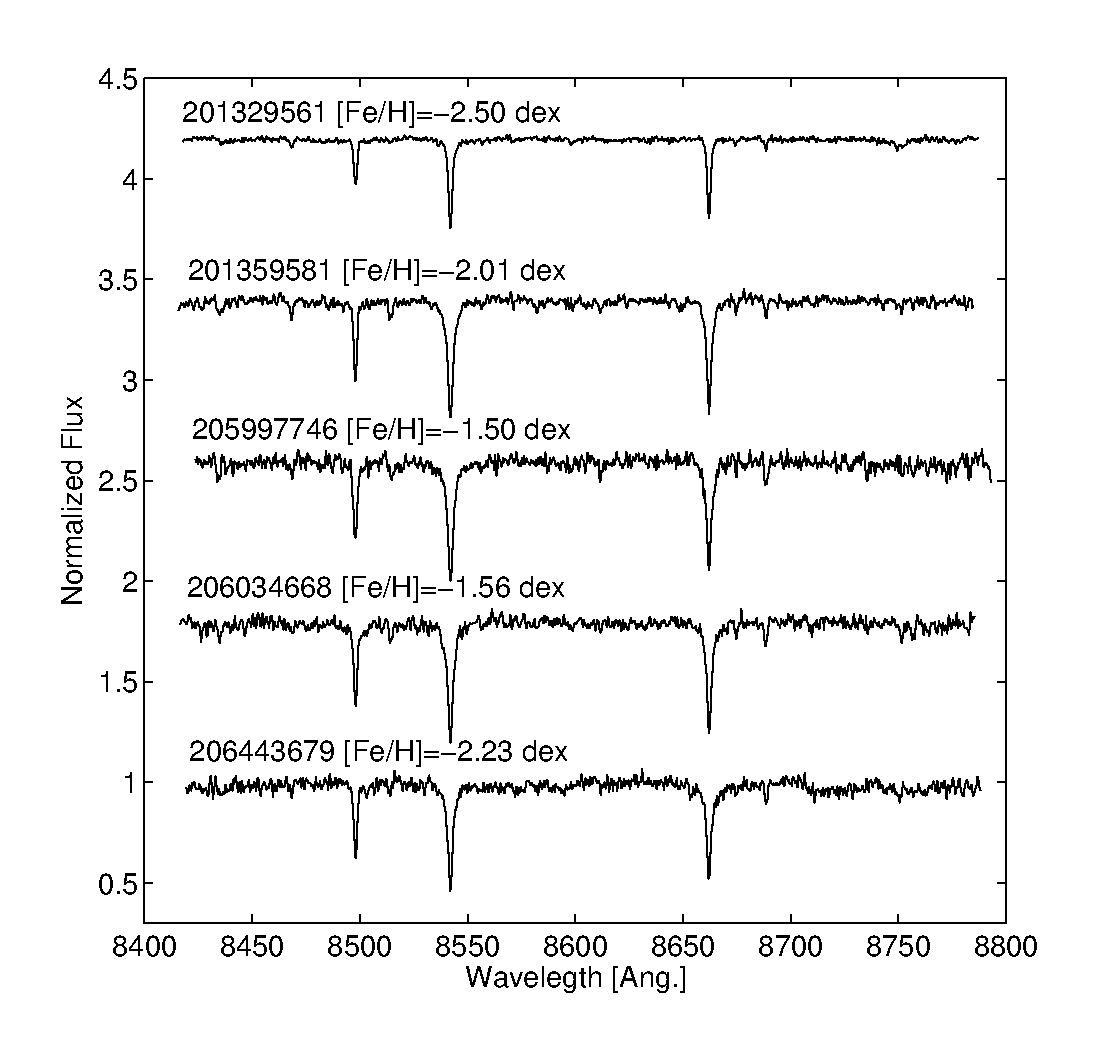
\includegraphics[width=1\columnwidth]{./Figures/spectra.pdf}
   \caption{RAVE spectra of the 4 metal-poor stars presented in this paper. Spectra are normalized and corrected for radial velocity, the Fe content labeled comes from the analysis of RAVE spectra using the same method as in \cite{Valentini2017}.}
              \label{Fig:spectra}%
    \end{figure}
%-------------------------------------------Spectra

%-------------------------------------- Spectro
   \begin{figure}
   \centering
   \includegraphics[width=1\columnwidth]{./Figures/Figure2.pdf}
   \caption{Atmospheric parameters of the sample of metal-poor stars, as taken from literature and this work: RAVE spectra and seismic parameters (red squares), RAVE-DR5 (blue triangles), RAVE-on (cyan triangles) and ESO high-resolution spectra and seismic parameters (black circles). }
              \label{Fig:datalit}%
    \end{figure}
%-------------------------------------- Spectro
%--------------------------------------TSNE
   \begin{figure}
   \centering
   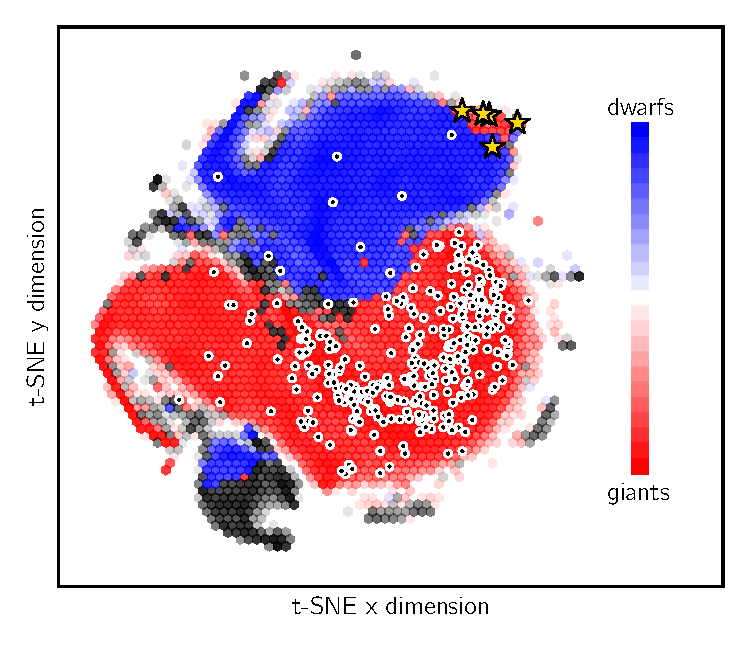
\includegraphics[width=1\columnwidth]{./Figures/Tsne.pdf}
   \caption{t-SNE projection of $\sim$420,000 RAVE spectra. The scaling in both direction is arbitrary,
therefore the units on the axes are omitted. The colour scale corresponds to the gravity of the
stars as computed by \citet{Kunder2017}. Giants are shown in red and dwarfs in blue. Lighter shaded hexagons include fewer stars than darker ones. Over-plotted black dots indicate locations of RAVE stars in K2 Campaigns 1,3; over-plotted stars indicate RAVE-K2 stars falling in the metal-poor locus, those stars correspond to the 4 stars analysed in this paper.\Marica{Gal can do the figure with 4 stars instead of 5.}}
              \label{Fig:Tsne}%
    \end{figure}
%--------------------------------------TSNE
The t-SNE analysis of \cite{MAt2017} mentioned before identified the stars presented in this paper as metal poor stars. Fig.~\ref{Fig:Tsne} shows a diagram of the 2-dimensional t-SNE projection \citep{van2008visualizing} of $\sim$420,000 RAVE spectra with SNR > 10 , with the RAVE stars in K2 C1 and C3 represented as empty circles. There are five stars that fall onto the very metal-poor island (top right) that corresponds to the 5 metal poor giants of this work. \Marica{Figure need to be updated.}
%-------------------------------------- Seismo different pipelines
\begin{figure*}
\centering
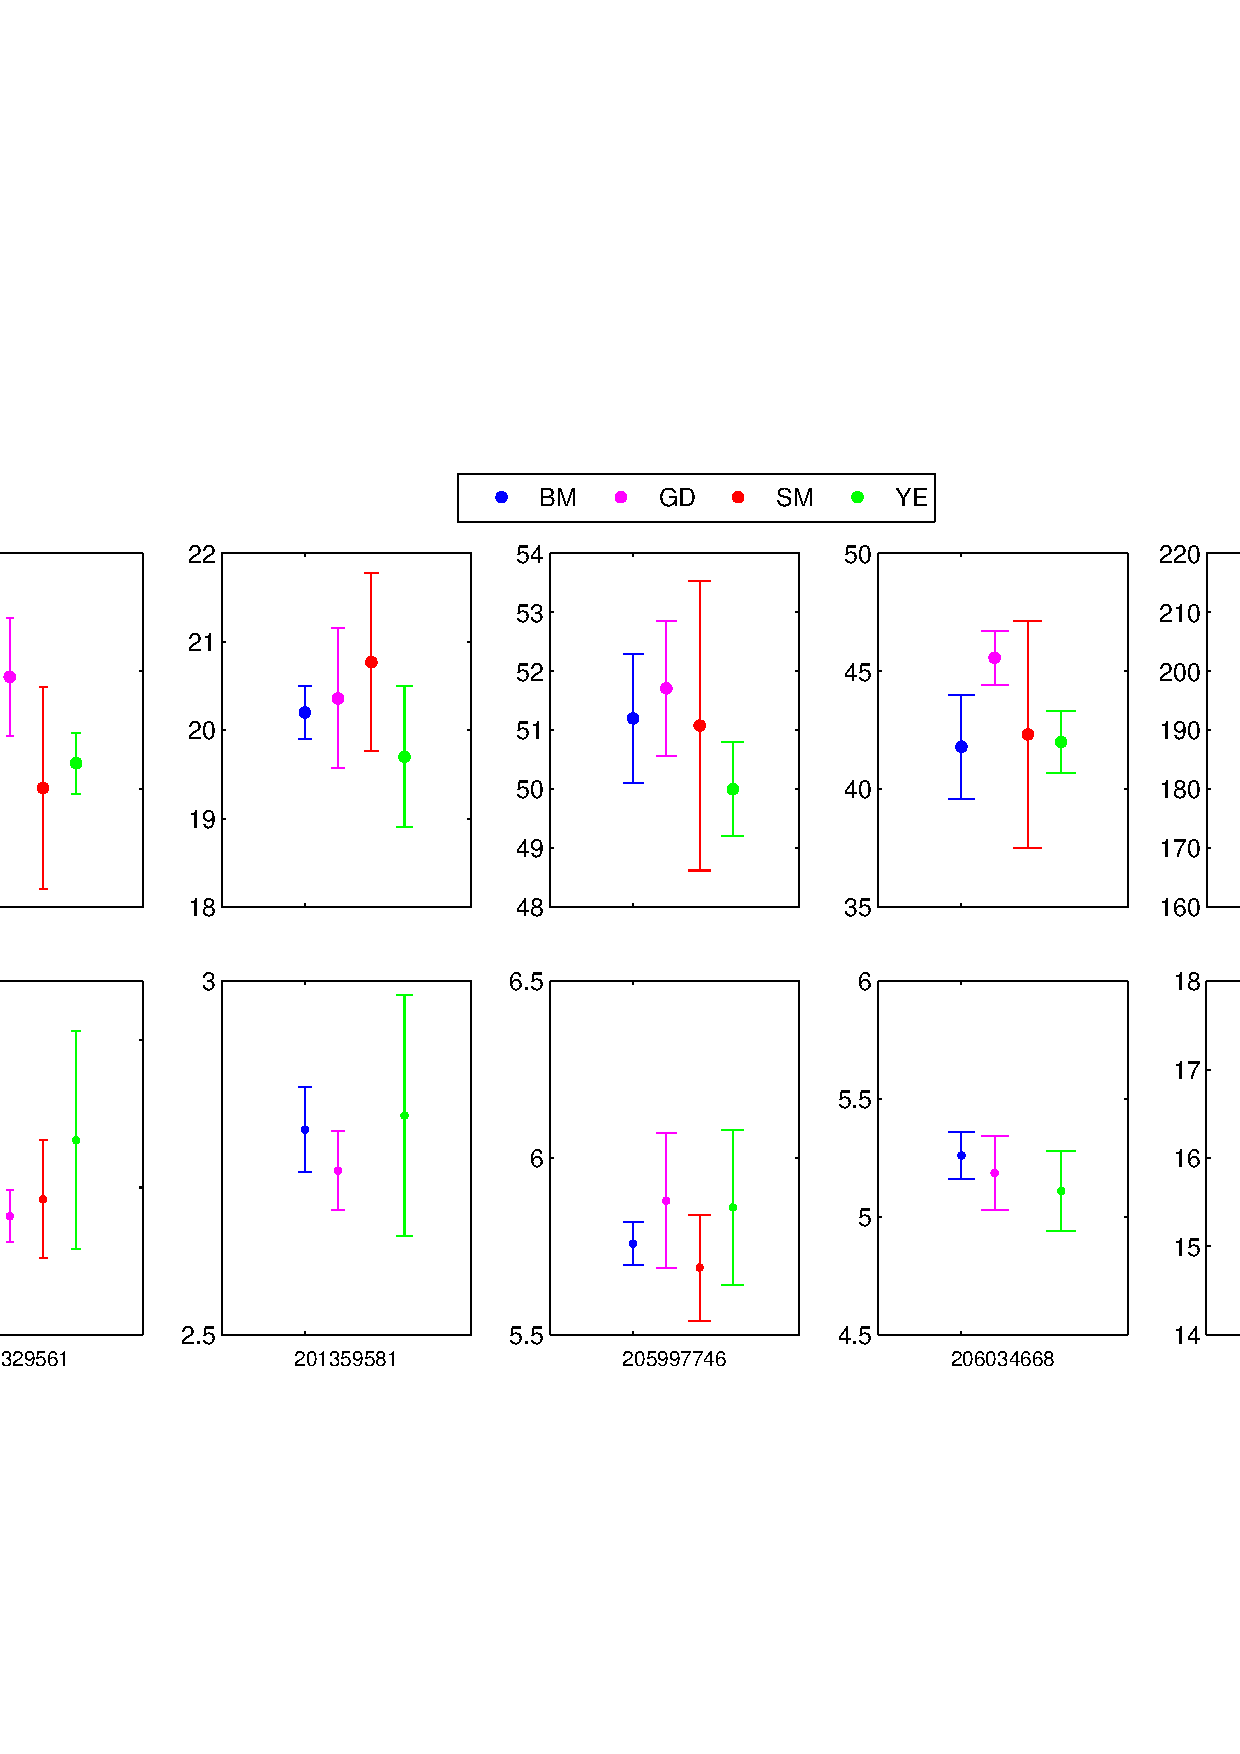
\includegraphics[width=1.7\columnwidth]{./Figures/dnunumax.pdf}
\caption{\Dnu and \numax as measured by different pipelines. Each colour (blue, magenta, red and green) corresponds to a different pipeline (B. Mosser, G. Davies, S. Matur and Y. Elsworth). The values plotted in black correspond to the values adopted for this work (BM$\_$N). }
\label{Fig:seismopipelines}%
\end{figure*}
%--------------------------------------------------
Light curves were obtained using the same approach described in \cite{Valentini2017}. In order to take into account the uncertainties in the seismic parameters, we considered the \deltanu and \numax measured by 4 different pipelines, identified as the initial of their first author \Marica{need some help here, 1 short sentence per method}:
\begin{itemize}
\item {\bf BM} It is the same method used for CoRoT and \kepler stars\citealp{Mosser2009, Mosser2011}. First the average frequency separation, \dnu , is measured from the autocorrelation of the time series computed as the Fourier spectrum of the filtered Fourier spectrum of the signal. The significance of the \Dnu is then checked using a statistial test based on the H0 hypothesis. If the \Dnu is reliable, then the other seismic parameters are measured with a technique that uses the expected frequency pattern of a Red Giant for identifying oscillations modes. 
\item {\bf GD} This pipeline is based on fitting a background model to the data \citep{Davies2016}. The model is a  model H \citep{Kallinger2014}, comprised of two Harvey profiles, a Gaussian oscillation envelope, and an instrumental noise background. For the estimate of \Numax the central frequency of the Gaussian component is considered. The median and the standard deviation are used to summarize the normal-like posterior probability density for \numax. To estimate the average frequency separation, the same method of BM have been used.
\item {\bf YE} This is a three stages approach \cite{Elsworth2017}. First, a signal-to-noise ratio spectrum (SNR) in function of frequency is created by dividing the power spectrum by a heavily smoothed version of the raw power spectrum. The second step consists in using a combination of H0 and H1 hypothesis for decting oscillation power in segments of the SNR spectrum. If a segment shows detection of oscillations power, then \Numax and \Dnu are detected as a third step\cite{Hekker2010}. This pipeline provided \Dnu with an uncertainty larger that the one provided by other pipelines.
\item {\bf SM} A first esimate of \Dnu was done using the same method as BM. \numax is measured by fitting a Gaussian on top of the background to the power spectrum. Then \Dnu is recomputed from the power spectrum of the power spectrum and by considering only the central orders of the spectrum centered on the highest radial mode \citealp{Mathur2010, Mathur2011}. Differently from the previous pipelines, this one measured a value for \Dnu only for 2 of the 4 targets and provided significantly larger errorbars for \numax.
\end{itemize}

In our analysis we adopter the values of BM, considering their internal error plus an external error, computed as the dispersion between the four pipelines. \Marica{Some seismo expert here: a sentence explaining WHY we chose BM is needed.} The adopted values are listed in Table~\ref{Tab:seism} and visible in Fig.~\ref{Fig:seismopipelines}. We compared the \deltanu and \numax of our sample with the  \deltanu and \numax distribution of APOGEE-{\it Kepler} targets (cita), as visible in Fig.~\ref{Fig:dataseismo}. Using {\it Kepler} stars as reference, our stars fall in the area of the distribution where the less massive stars are located.    
%-------------------------------------- Seismo
   \begin{figure}
   \centering
   \includegraphics[width=1\columnwidth]{./Figures/HRdiag.pdf}
   \caption{Position in the temperature - luminosity diagram of the 4 stars of this work (nomenclature following Table 1). Evolutionary tracks at Z=0.00022 and at different masses are plotted (M= 0.8, 0.9, 1.0 and 1.1 \Msun).}
              \label{Fig:tracks}%
    \end{figure}
%--------------------------

%HR spectroscopy
\subsection{High-resolution spectroscopic analysis}
UVES high resolution spectra of the 4 metal poor stars were collected in the period 99D, using UVES-CD23 setup, program ID: 099.D-0913(A). Spectra have a resolving power of $\sim$110,000 In Table \ref{Tab:ESO} are listed the observing date, exptime and SNR of spectra. 
%TABLE2----------------------------------------------------------------------------
\begin{table*}
\caption{Coordinates and set-up of the ESO-UVES observations of the stars. JD middle starts at 2017-05-16T09:29:09.314 (JD = 2457889.895247). The SNR listed is the one calculated in the all spectral range.}
\label{Tab:ESO}
\centering          
\begin{tabular}{lcccccc}     % 6 columns 
\hline\hline       
EpicID & RA & DEC  & JD middle & Setup & Exptime & SNR \\ \hline
201359581 & 178.650541 &  $-$1.56250& 57863.10762427578 & UVES-CD3 & 1200s & 60\\
205997746 & 339.990916 & $-$14.88894& 57941.21053530200 & UVES-CD3 & 3000s & 78\\
206034668 & 333.817541 & $-$13.83519& 57889.39524668500 & UVES-CD3 & 1300s & 70\\
206443679 & 338.755333 &  $-$5.90969& 57950.41013379906 & UVES-CD3 & 2600s &100\\
\hline
\end{tabular}
\end{table*}

	
	
	
	

%------------------------------------------------------------------------------------
We analysed spectra using the GAUFRE pipeline for retrieving \teff , \logg , and \FeH iteratively using the seismic information on \logg , adopting the seismic values listed in Table~\ref{Tab:seism}. Abundances of different chemical elements wete derived using MOOG 2017 \footnote{\url{http://www.as.utexas.edu/\%7Echris/moog.html}}, in the updated version treating Raylegh scattering properly (\cite{Sobeck2011} version available in github \footnote{Github link: \url{https://github.com/alexji/moog17scat}}). 

The linelinst was constructed using linelist presented by Roederer et al 2014, XXX et al 2017 and VALD DR4 (cite). In the following paragraph we will discuss the choice of line parameters and NLTE and 3D effects.

3D effects blabla. Not discussed here.

\textit{Carbon}. C abundance was derived via fitting the A-X CH bandhead at $\sim$4000-4300 \AA. Line parameters from XXX. 

\textit{Nitrogen}. From CN band.

\textit{Oxygen}. Where detectable.

\textit{Alpha-elements}. From ESO spectra we measured the abundances of Mg, Si, Ca and Ti. From the lines. NLTE corrections for Ti are taken from the work of \cite{NLTETi}.

\textit{Iron peak}. We measured abundances of Cr, Mn, Fe, Ni, Cu, Zn , and Ga. For Fe we adopted the line-by-line NLTE corrections provided by \cite{NLTEFe}. NLTE corrections for Mn are taken from \cite{NLTEMn}. Line-by-line corrections for Fe and Mn are taken from an user-friendly inteface available online \footnote{Available at the website \url{http://nlte.mpia.de/}}.

\textit{n-capt elements}. We were able to measure the element abundances of r- and s- process elements. As indicator of r-process enrichment we measured abundances of Eu, Gd, Tb, and Dy. As s-process markers we measured Sr, Ba and Ce.  

Final abundances and atmospheric parameters are listed in Table~\ref{Tab:stars}. The adopted linelist and the EW of every line used are listed in the Appendix (or online material?).
\begin{table*}
\caption{Atmospheric parameters and chemical abundances derived for the 4 metal-poor stars presented in this work. Values were derived from UVES spectra via EW or line fitting.}
\label{Tab:abundances}
\centering          
\begin{tabular}{ll|ccc|ccc|ccc|ccc|c}     % 15 columns
\hline  \hline 
      &  &   \multicolumn{3}{|c|}{201359581} &  \multicolumn{3}{|c|}{205997746} &  \multicolumn{3}{|c|}{206034668} &  \multicolumn{3}{|c}{206443679}&  \\ \hline
At. Par. &  &  &  &   &  &  &  &  &  &  & & & & \\ \hline
\Teff  & [K]  & &4850   & 43   & & 5020 & 35  & & 4995 & 25 & & 5245& 35& \\ 
\Logg  & [dex]& &2.17   & 0.03 & & 2.58 & 0.02& & 2.58 & 0.04& & 3.17& 0.05& \\
vmic   & [km/s]& &2.1   & 0.5  & & 1.80  & 0.5 & & 2.40& 0.4& & 1.8 & 0.5 & \\ \hline
Species & At. N. &  Nlin&   Abd  &  eA  &  Nlin  & Abd. & eA &  Nlin  & Abd. & eA  &  Nlin  & Abd. & eA & Met.\\ \hline
C    & 6.0    &      & 6.92   & 0.15  &   & 6.94 & 0.10 &   & 7.08 & 0.11 &   & 6.48 & 0.09 & f \\
Na I &11.0    & 2    & 7.31   & 0.12  & 2 & 6.07 & 0.12 & 2 & 4.96 & 0.05 & 2 & 4.68 & 0.08 & ew \\
Mg I &12.0    & 3    & 6.24   & 0.11  & 3 & 6.92 & 0.05 & 3 & 6.34 & 0.15 & 3 & 6.36 & 0.10 & ew \\
Si I &14.0    & 2    & 6.45   & 0.07  & 2 & 6.81 & 0.03 & 2 & 6.60 & 0.10 & 2 & 6.36 & 0.10& ew \\
Ca I &20.0    &  7   & 5.01   & 0.05  & 7 & 5.45 & 0.10 & 7 & 5.05 & 0.13 & 7 & 4.95 & 0.13 & ew \\
Sc II&21.1    &  3   & 1.66   & 0.11  & 3 & 1.84 & 0.14 & 3 & 1.74 & 0.11 & 3 & 1.53 & 0.14 & ew \\
Ti I &22.0    &  11  & 3.40   & 0.08  & 11& 3.91 & 0.15 & 9 & 3.59 & 0.10 & 11& 3.58 & 0.10 & ew \\
Ti II&22.1    &  17  & 3.56   & 0.10  & 17& 3.95 & 0.11 & 16& 3.68 & 0.12 & 17& 3.60 & 0.09 & ew \\ 
Cr I &24.0    &   9  & 3.84   & 0.22  & 9 & 4.38 & 0.11 & 7 & 3.98 & 0.09 & 9 & 3.87 & 0.09 & ew \\
Cr II&24.1    &      &        &       & 2 & 4.70 & 0.08 & 2 & 4.04 & 0.08 & 2 & 4.18 & 0.07 & ew \\ 
Mn I &25.0    &  1   & 3.69   & 0.08  & 1 & 4.32 & 0.10 & 1 & 3.82 & 0.09 & 1 & 3.48 & 0.08 & ew \\ 
Fe I &26.0    & 69   & 5.73   & 0.11  & 68& 6.14 & 0.10 & 67& 5.99 & 0.12 & 63& 5.37 & 0.10 & ew  \\
Fe II&26.1    & 10   & 5.82   & 0.10  & 9 & 6.12 & 0.09 & 7 & 6.03 & 0.10 & 7 & 5.51 & 0.12 & ew \\
Ni I &28.0    & 3    & 4.57   & 0.10  & 3 & 5.08 & 0.09 & 3 & 4.67 & 0.11 & 3 & 4.49 & 0.07 & ew \\  
Cu I &29.0    & 1    & 2.19   & 0.07  & 1 & 3.06 & 0.10 & 1 & 2.49 & 0.08 & 1 & 2.03 & 0.10 & ew \\                           
Zn I &30.0    & 2    & 3.05   & 0.11  & 2 & 3.51 & 0.11 & 2 & 3.42 & 0.14 & 2 & 3.00 & 0.11 & ew \\  
Ga I &31.0    &     &   &   & & & & & & & & & & f \\                        
Sr I &38.0    &     &   &   & & & & & & & & & & f \\                            
Ba II&56.1    &  2   & $-$0.60& 0.08  &3 & $-$0.07 & 0.09& 2 & 0.61& 0.10 & 2 & $-$0.45& 0.13 & f \\ 
Ce II&58.1    &     &   &   & & & & & & & & & & f \\ 
Pr II&59.1    &     &   &   & & & & & & & & & & f \\ 
Nd II&60.1    &     &   &   & & & & & & & & & & f \\ 
Sm II&62.1    &     &   &   & & & & & & & & & & f \\  
Eu II&63.1    &     &   &   & & & & & & & & & & f \\
Gd II&64.1    &     &   &   & & & & & & & & & & f \\
Tb II&65.1    &     &   &   & & & & & & & & & & f \\                            
Dy II&66.1    &     &   &   & & & & & & & & & & f \\ \hline
\end{tabular}
\end{table*}

%-------------------------------------- Seismo
   \begin{figure*}
   \centering
   \includegraphics[width=1.99\columnwidth]{./Figures/RAVEMP_chempat.pdf}
   \caption{Chemical pattern of the 4 stars, as [X/Fe] \Marica{this figure will be upgraded any time a new element will be measured.}}
              \label{Fig:abdpattern}%
    \end{figure*}
%-------------------------------------- Seismo
%-------------------------------------- Seismo
   \begin{figure}
   \centering
   \includegraphics[width=0.99\columnwidth]{./Figures/DnuNumax_2.pdf}
   \caption{\Dnu and \numax distribution of the 5 stars studied in this work. On the background the \dnu-\numax distribution distribution of the APOKASC sample (cita paper Thaise), colour coded following the mass.}
              \label{Fig:dataseismo}%
    \end{figure}
%-------------------------------------- Seismo

%-------------------------------------- PDF
   \begin{figure*}
   \centering
   \includegraphics[width=2\columnwidth]{./Figures/relative_MassAge.pdf}
   \includegraphics[width=2\columnwidth]{./Figures/relative_MassAge2.pdf}
   \caption{Top: Mass-\FeH (left) and age-\FeH (right) distribution for the set of stars of this work calculated using PARAM with MESA tracks and RAVE atmospheric parameters. Each colour represent mass and ages derived using different approaches, as specified in the legend. Each set of data is coded as PPXXaAA, where the string ''PP'' is the seismic pipeline that provided \dnu and \numax (BM, GD, YE and SM), ''XX'' is the $\eta$ value (0.2 or 0.4) and ''AA'' is the [$\alpha$/Fe] (00=0.0 dex, 01=0.1 dex, etc). Bottom: Mass-\FeH (left) and age-\FeH (right) distribution for the set of stars of this work calculated using PARAM with MESA tracks and ESO spectra atmospheric parameters. Same nomenclature as top figure but here only one alpha enhancement, corresponding to the measured one, have been considered \Marica{And S1 was removed: It seems that things changed al lot. Do I have to add errorbars?}.}
              \label{Fig:relative}%
    \end{figure*}
%--------------------------------------

\section{Mass and age determination}
\label{Sect:massage}


%-------------------------------------- PDF
   \begin{figure}
   \centering
   \includegraphics[width=0.99\columnwidth]{./Figures/ViolinBM02alpha0203.pdf}
   \caption{Violin plot illustrating the probability distribution functions of the mass and age of the stars in this work, derived using PARAM.}
              \label{Fig:violin}%
    \end{figure}
%--------------------------------------

%TABLE3----------------------------------------------------------------------------
\begin{table*}
\caption{Seismic mass, radius and distances calculated using scaling relations, and mass,radius, and age derived using PARAM, for the 4 metal-poor RAVE stars in K2 Campaigns 1 and 3. \Marica{S1 need to be taken out. Figure need to be updated with the latest results.}}
\label{Tab:seismres}
\centering          
\begin{tabular}{lccccccc}     % 13 columns 
\hline\hline       
EpocID & Mass$_{\rm scaling}$ & Radius$_{\rm scaling}$ & Mass$_{PARAM}$ & Radius$_{PARAM}$ & Age$_{PARAM}$  \\
 & [\msun] & [\rsun]  & [\msun] & [\rsun] & [Gyr]  \\  \hline
201359581 & 1.323$\pm$0.187 & 14.337$\pm$0.158 & 0.7922$^{0.9508} _{0.7798}$& 13.521$^{+1.836} _{-0.639}$ & 13.0040$^{13.9593} _{7.3892}$  \\
205997746 & 1.114$\pm$0.064 & 8.352$\pm$0.077 & 1.0538$^{1.2301} _{0.8191}$ & 7.897$^{+0.381} _{-0.294}$ & 7.8440$^{12.7090} _{3.1261}$  \\
206034668 & 0.865$\pm$0.107 & 8.153$\pm$0.204 & 0.7989$^{0.8774} _{0.7870}$ & 8.018$^{+0.415} _{-0.191}$ & 13.200$^{13.9601} _{9.8605}$  \\
206443679 & 1.001$\pm$0.135 & 4.079$\pm$0.156 & 0.8604$^{0.9289} _{0.7953}$ & 3.909$^{+0.186} _{-0.125}$ & 9.8707$^{12.7365} _{7.6736}$  \\
\hline
\end{tabular}
\end{table*}
%------------------------------------------------------------------------------------

%-------------------------------------- PDF
   \begin{figure}
   \centering
   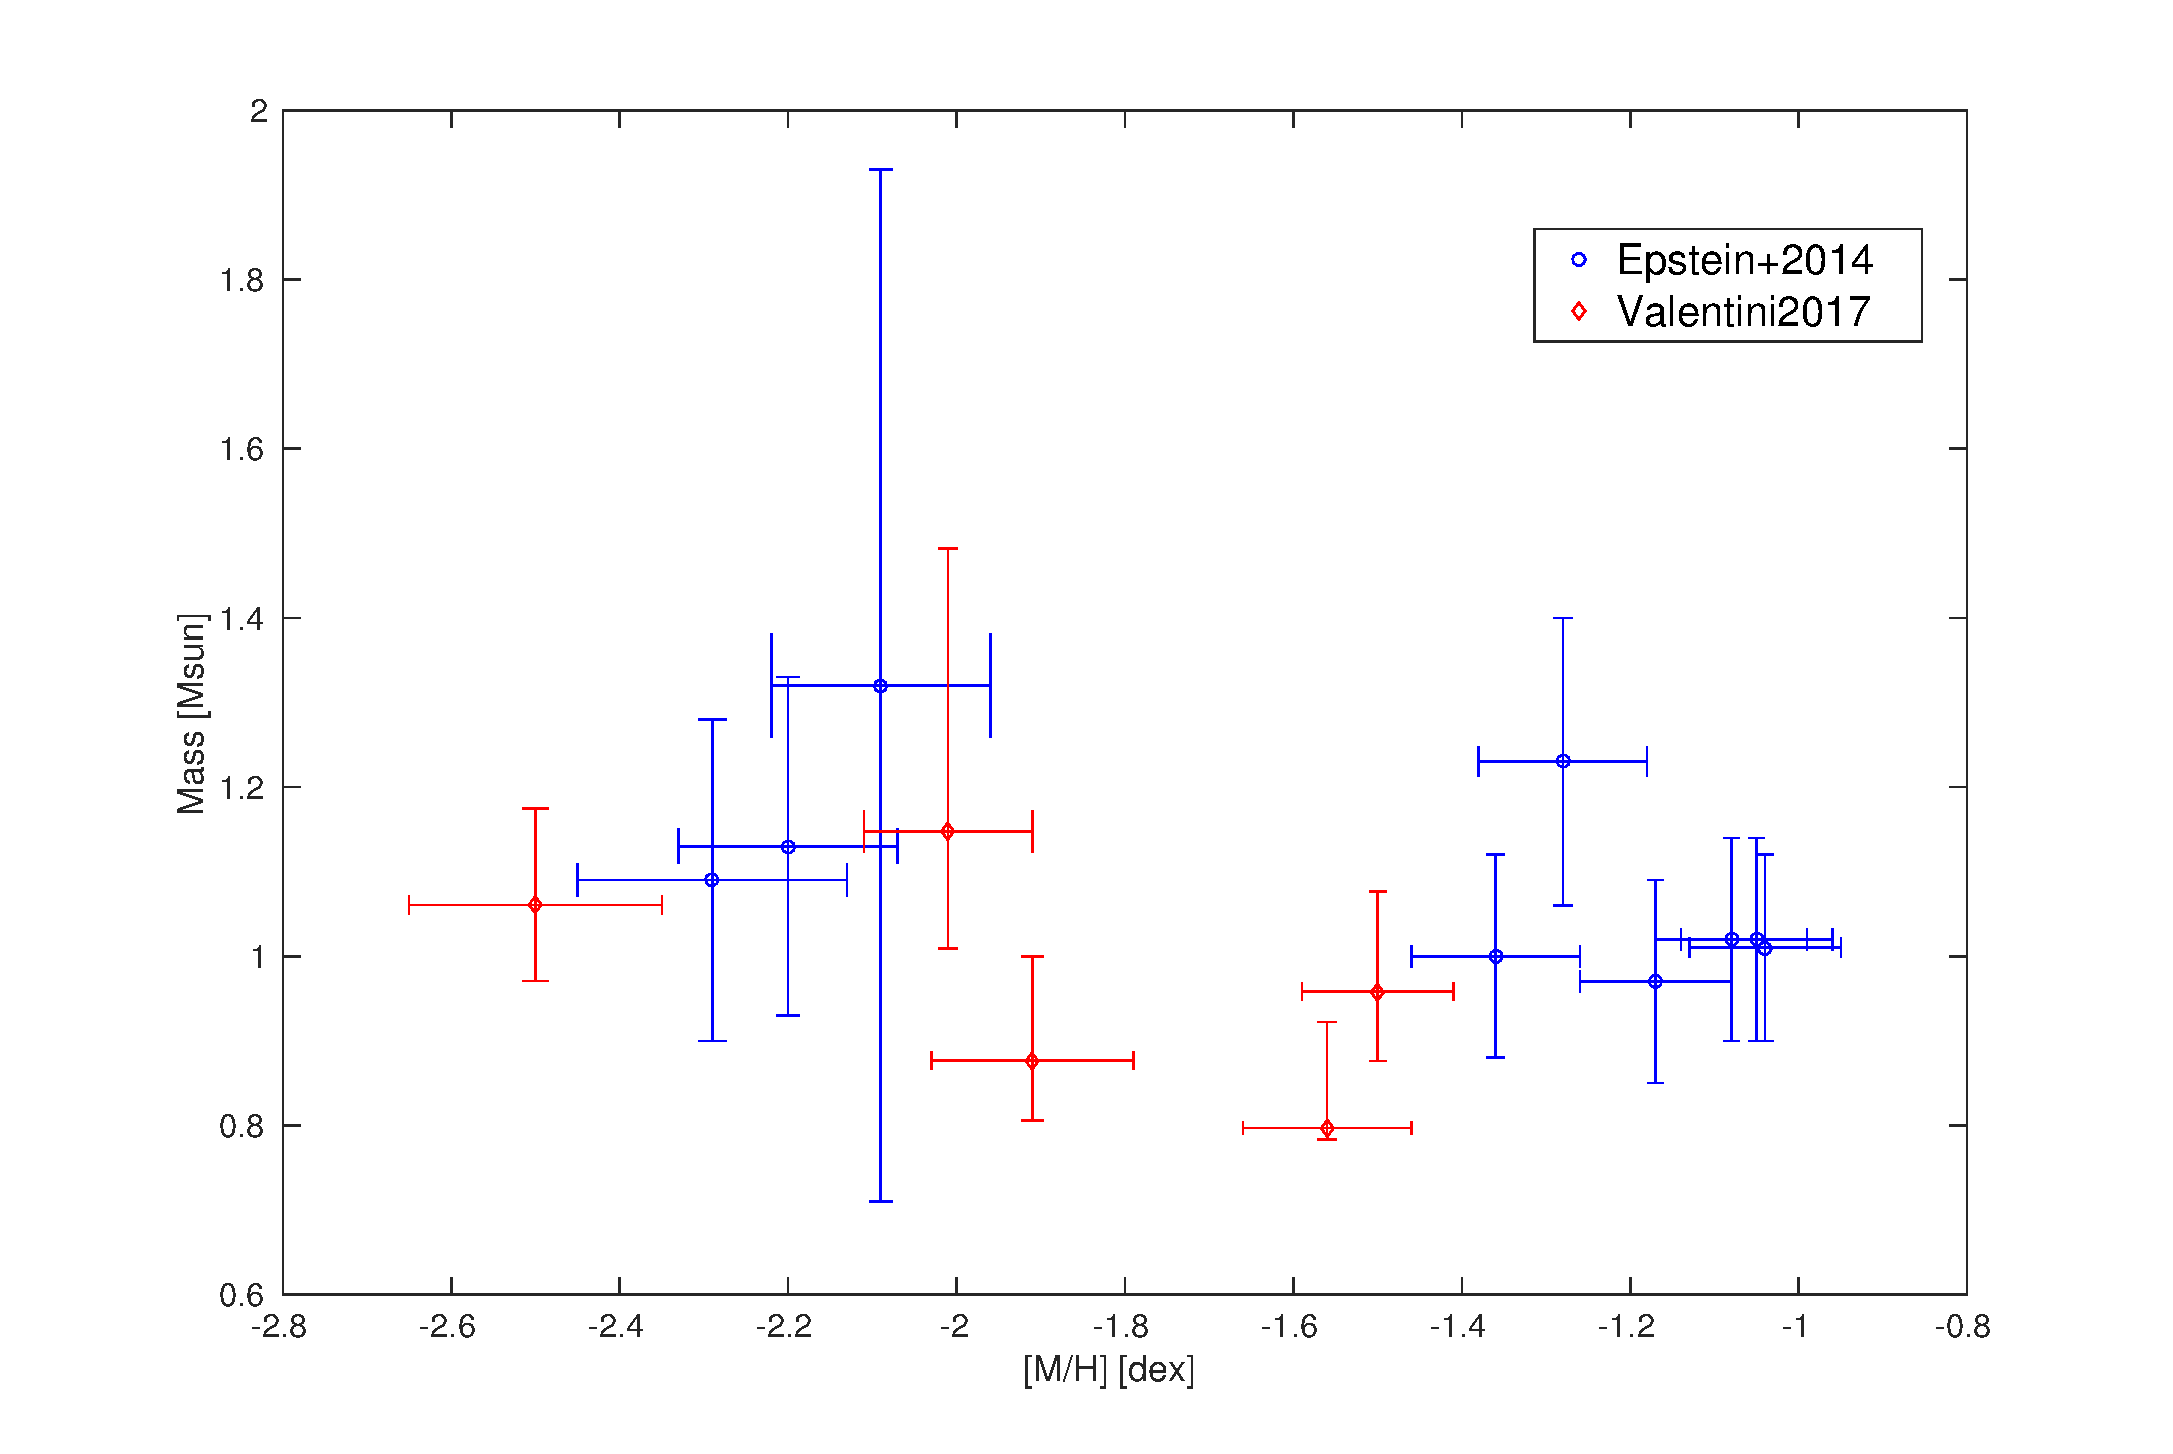
\includegraphics[width=1.0\columnwidth]{./Figures/Epstein.pdf}
   \caption{Mass and metallicity distribution of the 4 stars presented in this work (red points) and the object of the work of \cite{Epstein2014}. Old \cite{Epstein2014} values are plotted as empty circles, the recomputed values using PARAM (same as the stars in this work) are plotted as blue diamonds. \Marica{Figure updated.}}
              \label{Fig:Epstein}%
    \end{figure}
%--------------------------------------

Mass determination have been per formed using two different methods: a direct method, using scaling relations, and via Bayesian fitting  using the PARAM code. 

%Paragrafo PARAM 
For deriving ages and masses of our stars we adopted the latest version of the PARAM code \citep{2017MNRAS.467.1433R}. The new version of the code uses \dnu and \numax that have been computed along the evolutionary tracks (the previous version was using the frequencies inferred using scaling relations). Respect to the version described in \citep{2017MNRAS.467.1433R}, we extended the grid towards the metal poor end, up to [Fe/H]=-3 dex, by calculating evolutionary tracks for \FeH = -2.0 and -3.0 dex, assuming the He enrichment formula as described in \citet{2017MNRAS.467.1433R}. We also took into account mass loss and $\alpha$-elements enrichment.

The values of stellar mass and radius, derived using scaling relations and PARAM, are shown in Tab.~\ref{Tab:seismres}. The error on the mass and radius derived using the direct method is calculated using propagation of uncertainties (under the assumption of uncorrelated variables). The mass and ages of PARAM are derived using a mass loss value of $\eta$=0.2: we adopted this value since it is in agreement to what measured in \cite{Miglio2012} by comparing the asteroseismic masses of Red Clump stars and Red Giants in the old open clusters NGC6791 and NGC6819. We also adopted an [$\alpha$/Fe]=0.3 dex, a value similar to what measured from RAVE spectra.  The error associated to radius, mass and age derived using PARAM is calculated as the 68 percentile of the PDF. The PDFs of mass and age of the objects of this work are shown in Fig.~\ref{Fig:violin}.

\subsection{Uncertainties}

In the age and mass determination we took always into account the uncertainties in the adopted  atmospheric parameters and the uncertainties in the \dnu and \numax determination.

For better understanding the systematics that may affect the age determination using PARAM, different seismic pipelines, and spectroscopic values, we performed several tests under different assumptions:
\begin{itemize}
\item We determined ages and masses for each set of seismic parameters provided by the 4 different pipelines.
\item  For each set of seismic parameters, we considered 5 different [$\alpha$/Fe] abundances, 0.0, 0.1, 0.2, 0.3, 0.4 dex. Since the low resolution and the limited wavelength interval of RAVE may affect the measured alpha content of the stars, we wanted to quantify the impact of a miscalculated [$\alpha$/Fe]. 
\item Two different mass loss approximations were considered, $\nu=$0.2 and 0.4. This test has been performed for each set of seismic data adopted.
\item A difference in temperature that may exist between different methods for measuring \Teff, as pointed out by {\bf [cite a paper]}. We determined mass and ages for the selected seismic parameters by varying the \Teff of $\pm$ 100 K. 
\end{itemize}
It is worth to remember that the effects of these tests depend on the position of the star on the HR diagram, and on its evolutionary stage. Each locus of the HR diagram is populated by different tracks and with different levels of degeneracy. 

The variation on $\alpha$ content has no significant effect, providing a mass spread on average of 0.01 Msun and of 0.3 Gyrs in age. As a general behaviour, when the $\alpha$ enrichment increases the mass slightly decreases (and the age increases). 

The underestimation of \Teff lead to a variation in mass and age on average of XX and XX respectively. An overestimation of the same amount leads to a variation of XX in mass and XX in age. When temperature increases the mass increases and the age decreases, the contrary happens when the temperature decreases. This effect is more visible for the most metal poor and hottest stars.

The adoption of a mass loss parameter $\eta$=0.4 leads to a mass and age spread of only XX and XX in mass and age respectively. As discussed in \cite {Anders2016} and \cite{Casagrande2016}, the effect of mass loss is more significant for red clump stars than for RGB stars.

Fig.~\ref{Fig:relative} shows the mass-\FeH and the age-\FeH distributions for every set of calculations we performed. Masses and ages coming from the same calculation had been connected with a line in order to facilitate the reading of the figure (except for the calculations performed using SM seismic parameters, where PARAM converged only for 2 stars). It is visible how the bigger impact on age and mass comes from the seismic parameters, while the [$\alpha$/Fe] and mass loss have a minor effect. The different approaches in seismic parameter pipelines, $\alpha$ content and mass loss do not alter the relative ages of the stars. The mass and ages determined using the seismic values coming from every single pipeline are showed in the Appendix, Fig.~\ref{Fig:agesBenoit},Fig.~\ref{Fig:agesGuy},\ref{Fig:agesSavita} and \ref{Fig:agesYvonne} for the two mass loss assumptions and the 5 different $\alpha$ content. The $\Delta$ \Teff tests using the \dnu and \numax adopted in this work are present in Appendix Fig.~\ref{Fig:Benoitalltests}. 

\section{Distance and orbits} 
Distances were calculated using PARAM and, when available, Gaia parallaxes.

Orbit parameters were calculated uing GALPY (Bovy, citaz. and link). We adopted a Galactic potential, a solar radius of X and soler proper motions from X and Y. Errors on orbit parameters were calculated via Monte-Carlo approach, simulating 1,000 stars per object  with velocity, distance and proper motions variating within errors. Results are summarized in Table~\ref{Tab:orbits}.

\begin{table*}
\centering
\begin{tabular}{llrrrrrrrrrr}
\hline \hline
ID & Dist.& Vrad. & PMRA & PMDE & U & V & W &  Rmin & Rmax & ecc & Zmax \\ 
   & Kpc  & kms   & mas/yr & mas/yr & Km/s & Km/s & Km/s & Kpc  & Kpc &   & Kpc   \\ \hline
S2 & 1.403& 77.140 & $-$51.2 $\sigma$= 0.9 & $-$4.7 $\sigma$= 1.0 & $-$346.222 &$-$251.59 & $-$45.19& 0.49 & 35.48 & 0.97 & 21.08 \\
S3& 1.871& $-$205.073 &  13.5 $\sigma$=1.1 & $-$2.6 $\sigma$=1.2 & $-$169.41& $-$134.95 &  106.02&   2.60 & 11.29 & 0.62 & 8.97 \\
S4& 1.386& 55.748 &  $-$24.2 $\sigma$=1.9 &$-$49.3 $\sigma$=1.4  &  428.85& $-$400.34& $-$55.51&    1.98 & 338.27 & 0.98 & 193.54 \\
S5& 0.698& $-$40.667 &  28.9 $\sigma$=1.1 & $-$0.7 $\sigma$=1.1  & $-$268.80&$-$101.39 & $-$126.38&   1.30 & 24.76 & 0.89 & 8.32 \\ \hline
\end{tabular}
\caption{Distance, radial velicity, proper motions and orbit parameters of the stars in this work. Distance has been derived by PARAM, using seismic parameters; radial velocity has been measured from ESO spectra via cross-correlation and proper-motions were taken from UCAC5 catalogue. Orbits have been integrated using Galpy using the MWpotential2014 potential.}
\label{Tab:orbits}
\end{table*}


\section{Discussion} 

\subsection{201359581}
This star belong to K2 Campaign 1. It is the only star where the temperature derived from the high resolution spectrum is 380 K lower than the \Teff derived from the lower resolution RAVE spectrum and the Teff derived from the IRFM. We already noticed in Valentini et al 2017 that the IRFM tends to over-estimate temperatures at Teff>5000 K. This is probably due to the adoption of RAVE parameters as an imput in the IRFM of Casagrande et al for RAVE. This is then reflected to the measurements of GAUFRE using seismic parameters, since we adopted IRFM temperature as a prior with a flexibility of 200 K. {\bf [Is that too strong as an assumption? The IRFM is known to work well, BUT the IRFM of Casagrande for RAVE used DR5 atmospheric parameters on \logg and \FeH as imput for models.]}

This star has also very low \Dnu and \numax. This gives less confidence in mass and radius, so we recommend to take the age of this star with extreme caution. The star seem to stay above the RGB  bump. 

The star is not C enhanced: [C/Fe]= $+$0.12 dex. The star appears enhanced in Na: [Na/Fe]=$+$2.84 dex. This might be due to unresolved Na interstellar lines, that hampers the abundance measurement. \Marica{A more accurate inspection rejected some Na lines, so I feel more compfortable to lower the log(A)$_{\bf Na}$ to lower values and adopt it as an upper limit.} 

Is the star a typical halo star?

\subsection{205997746}
\Marica{One paragraph or two per star}
The star is not C enhanced.

The star is below the bump.

The star is alpha enhanced.

Is the star a typical halo star ? Orbit/chemistry/age. This star has a peculiar orbit, with v$\phi_{mean}$=$-$0.133 km/s. Can this star be an accreted object? What we can look at in the chemistry? It is the richest in Ba and the lowest in $\alpha$-elemnts content.

\subsection{206034668}
\Marica{One paragraph or two per star}
This star is rich in Ba.

The star is not C enhanced.

The star is below the bump.

The star is alpha enhanced.

Is the star a typical halo star ? Orbit/chemistry/age.

\subsection{206443679}
\Marica{One paragraph or two per star}

The star il alpha-enhanced.

The star is not C enhanced.

The star is below the bump.

Is the star a typical halo star ? Orbit/chemistry/age.


\subsection{Comparison with Epstein2014}
We compared the masses of our stars with the masses determined by the only work in literature that determines the masses of metal-poor stars, \cite{Epstein2014}. For the sake of homogeneity, we calculated again the masses of the Epstein sample using PARAM and the values provided in APOGEE-DR14. The recalculation of the masses led to smaller values respect to the original values (see Fig.~\ref{Fig:Epstein}) and our sample, together with the Epstein one, provides a better coverage of the [Fe/H] range $-$2.5-$-$1 dex.

\section{Conclusions}
\label{Sect:conclusions}

We determined mass and ages for a sample of 5 RAVE metal-poor stars. Our analysis took advantage of the seismic informations derived from K2 light curves (Campaigns 1 and 3): asteroseismology was first involved in the spectroscopic analysis and then in the mass and age determination using a Bayesian approach. All the stars but one, possess only intermediate resolution RAVE spectra, while only one target has been observed at higher resolutions. Abundances and atmospheric parameters available in literature for the known star are in agreement with the atmospheric parameters derived form RAVE spectra using the seismic \logg. Abundances and atmospheric parameters are summarized in Tables \ref{Tab:stars} and \ref{Tab:seismres}.

This exploratory work shows that asteroseismology is a powerful tool for determining masses and ages of stars. We derived masses and ages for the 5 RAVE metal poor stars, with a precision of XX\% and XX\% respectively. 

In the mass and age estimation process we thoroughly investigated the impact of different assumptions, and we concluded that:
\begin{itemize}
\item different seismic pipelines: 
\item Shifts in temperature:
\item $\alpha$:
\item Mass loss:
\end{itemize}
We concluded that for metal poor stars in the RGB phase an age determination based on relative ages is a safe approach. 

When available, we strongly suggest to use asteroseismology starting from the spectroscopic analysis, using the seismic \logg in an iterative way, as widely suggested by literature (e.g. Bathala, Morel, Valentini, Valentini). The resulting atmospheric parameters will be more consistent with the seismic parameters that are used for determining ages and masses. 

From our tests it is clear how an intensive study on the chronological chemical enrichment of the Halo is possible only if the sample of stars is analysed n an homogeneous way. At every step of the investigation, from the spectroscopic analysis to the mass and age determination, it is necessary to introduce the same seismic parameters and the same approach for every target. Only this can ensure a precise age and therefore a precise chronological characterization of the sample.

This work pave the path for a more extensive study of metal poor stars with asteroseismology: when combining the precise abundances from spectroscopy with the ages and masses provided by asteroseismology, it is possible to investigate chronologically the chemical enrichment of the Galactic halo. The forthcoming Gaia catalogues and spectra at higher resolution and wider spectral coverage will increase the precision and the number of the chemical abundances.

\begin{acknowledgements}
MV and CC acknowledge the DFG grant nr XXXXXX. AM, WJC, GRD, and YPE acknowledge the support of the UK Science and Technology Facilities Council (STFC). TSR acknowledges support from CNPq-Brazil. This work has made use of the VALD database, operated at Uppsala University, the Institute of Astronomy RAS in Moscow, and the University of Vienna. The authors acknowledge the International Space Science Institute (ISSI-Bern), that hosted the first AsteroSTEP meeting (\url{https://www.asterostep.eu}). Based on data obtained from the ESO Science Archive Facility under request number MVAL1980/265075. Funding for RAVE has been provided by: the Australian Astronomical Observatory; the Leibniz-Institut fuer Astrophysik Potsdam (AIP); the Australian National University; the Australian Research Council; the French National Research Agency; the German Research Foundation (SPP 1177 and SFB 881); the European Research Council (ERC-StG 240271 Galactica); the Istituto Nazionale di Astrofisica at Padova; The Johns Hopkins University; the National Science Foundation of the USA (AST-0908326); the W. M. Keck foundation; the Macquarie University; the Netherlands Research School for Astronomy; the Natural Sciences and Engineering Research Council of Canada; the Slovenian Research Agency; the Swiss National Science Foundation; the Science \& Technology Facilities Council of the UK; Opticon; Strasbourg Observatory; and the Universities of Groningen, Heidelberg and Sydney. The RAVE web site is at: \url{https://www.rave-survey.org}.
\end{acknowledgements}

% WARNING
%-------------------------------------------------------------------
% Please note that we have included the references to the file aa.dem in
% order to compile it, but we ask you to:
%
% - use BibTeX with the regular commands:
%   \bibliographystyle{aa} % style aa.bst
%   \bibliography{Yourfile} % your references Yourfile.bib
%
% - join the .bib files when you upload your source files
%-------------------------------------------------------------------

%\begin{thebibliography}{}
\bibliographystyle{aa}
\bibliography{RAVEMP}{}
%\end{thebibliography}

\begin{appendix}

    




%-------------------------------------- BM

\begin{figure*}
\centering
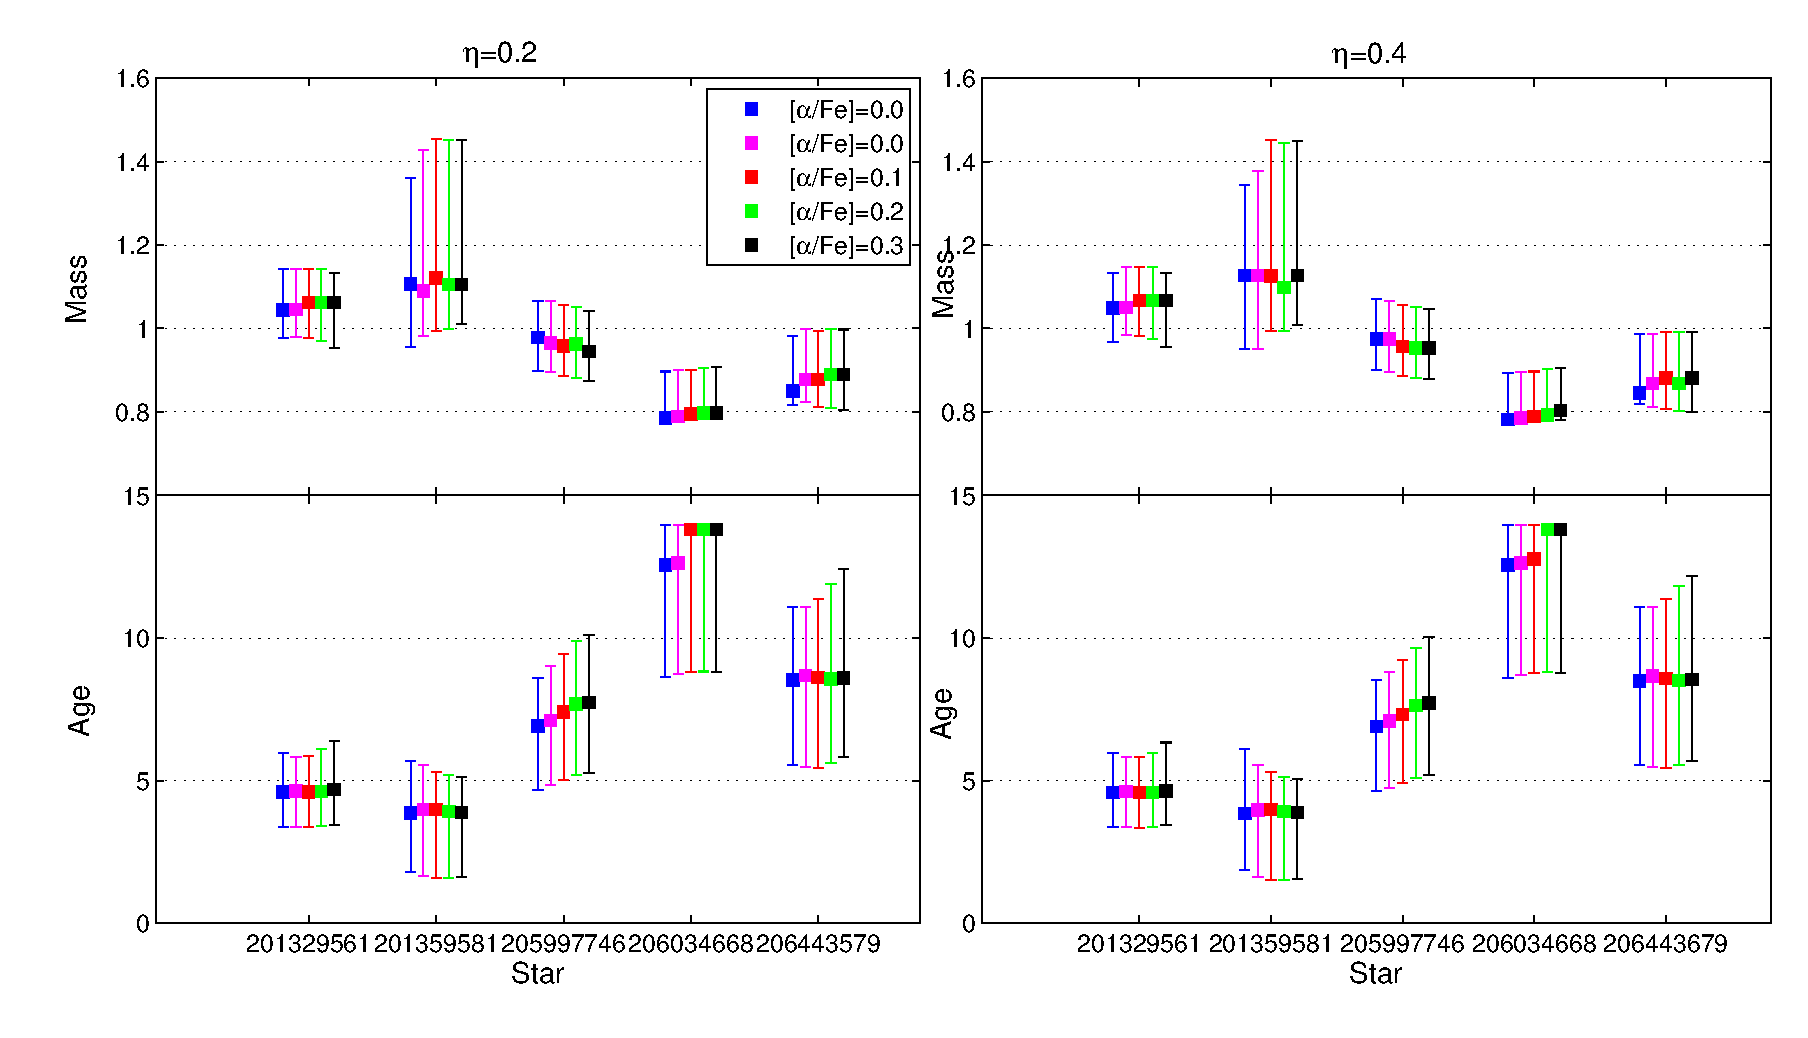
\includegraphics[width=1.7\columnwidth]{./Figures/Benoit.pdf}
\caption{Mass and ages of the 5 stars,determined using different [$\alpha$/Fe] (0.0,0.1,0.2,0.3,0.4 dex respectively) and two different $\eta$ parameters (0.2 and 0.4) for the mass loss. Benoit Mosser seismic parameters}
\label{Fig:agesBenoit}%
\end{figure*}

%-------------------------------------- GUY

\begin{figure*}
\centering
\includegraphics[width=1.7\columnwidth]{./Figures/GDagesMass.pdf}
\caption{Mass and ages of the 5 stars,determined using different [$\alpha$/Fe] (0.0,0.1,0.2,0.3,0.4 dex respectively) and two different $\eta$ parameters (0.2 and 0.4) for the mass loss. Guy Davies seismic parameters}
\label{Fig:agesGuy}%
\end{figure*}

%-------------------------------------- YVONNE

\begin{figure*}
\centering
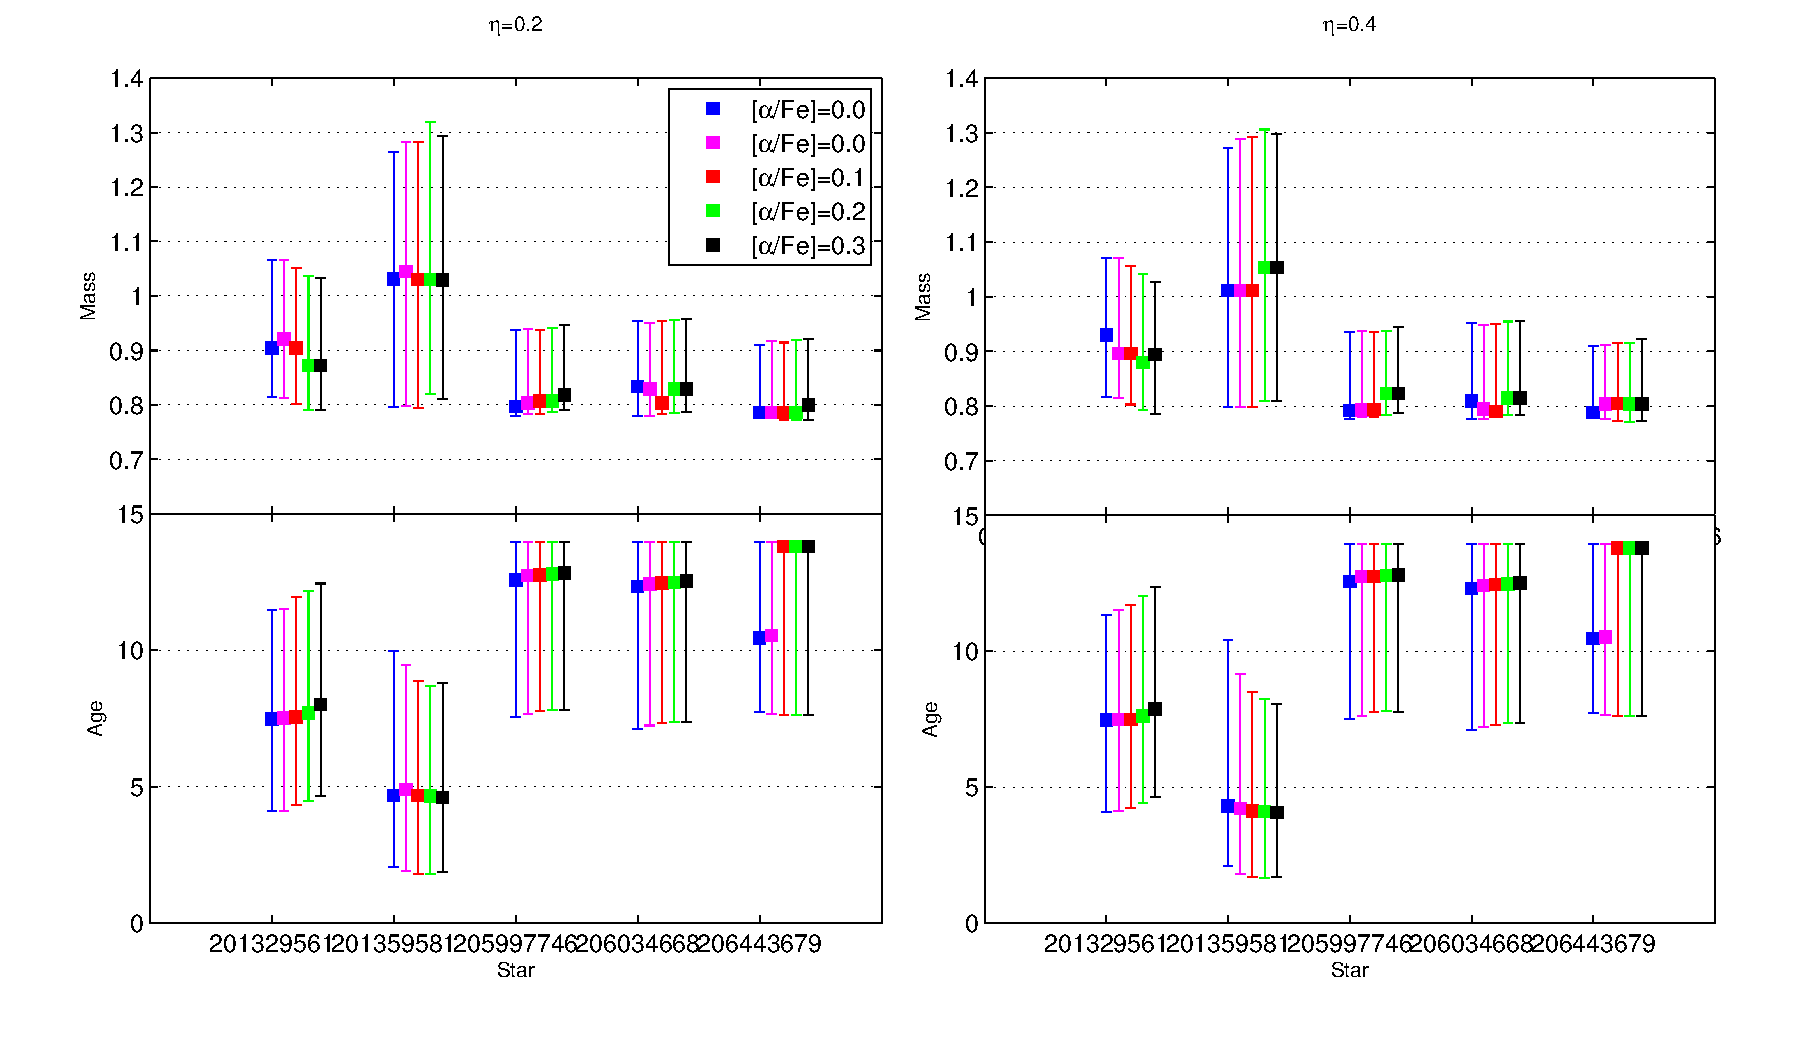
\includegraphics[width=1.7\columnwidth]{./Figures/agesYvonne.pdf}
\caption{Mass and ages of the 5 stars,determined using different [$\alpha$/Fe] (0.0,0.1,0.2,0.3,0.4 dex respectively) and two different $\eta$ parameters (0.2 and 0.4) for the mass loss.YVONNE ELSWORTH seismic parameters}
\label{Fig:agesYvonne}%
\end{figure*}

%-------------------------------------

%-------------------------------------- SAVITA
\begin{figure*}
\centering
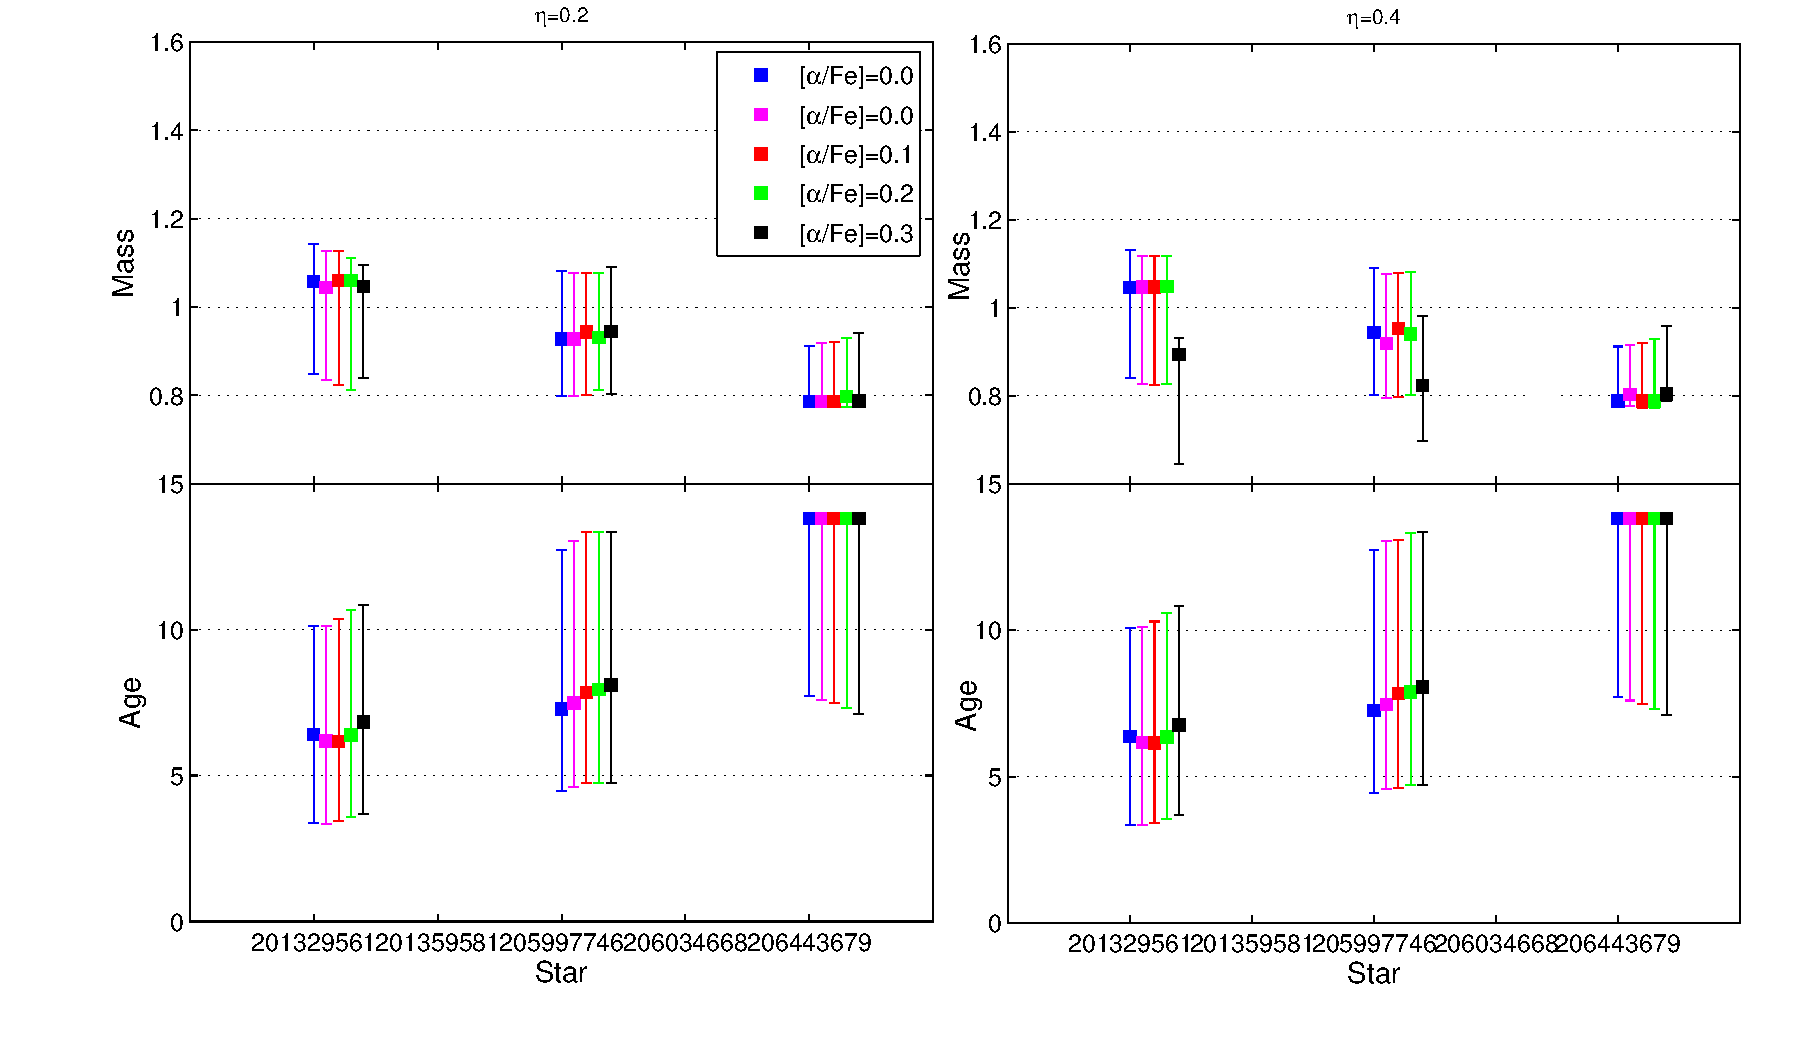
\includegraphics[width=1.7\columnwidth]{./Figures/agesSavita.pdf}
\caption{Mass and ages of the 5 stars,determined using different [$\alpha$/Fe] (0.0,0.1,0.2,0.3,0.4 dex respectively) and two different $\eta$ parameters (0.2 and 0.4) for the mass loss. SAVITA MATUR seismic parameters}
\label{Fig:agesSavita}%
\end{figure*}

%--------------------------------------



%-------------------------------------- Benoitalltests
   \begin{figure*}
   \centering
   \includegraphics[width=1.89\columnwidth]{./Figures/Mossernu02alltests.pdf}
   \caption{Mass and ages of the 5 stars,determined using different [$\alpha$/Fe] (0.0,0.1,0.2,0.3,0.4 dex respectively in blue, magenta, red, green and black) and varying the \Teff  of $\pm$100 K in each $\alpha$ assumption (triangle up for temperature increased, triangle down for decreased) .}
              \label{Fig:Benoitalltests}%
    \end{figure*}
%--------------------------------------



\end{appendix}
\end{document}
